

\tikzset{every picture/.style={line width=0.75pt}} %set default line width to 0.75pt        

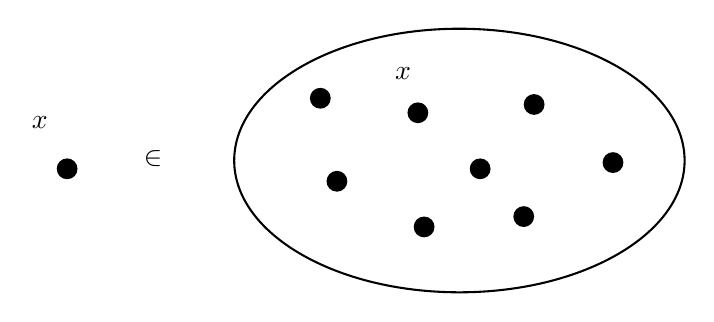
\begin{tikzpicture}[x=0.75pt,y=0.75pt,yscale=-1,xscale=1]
%uncomment if require: \path (0,300); %set diagram left start at 0, and has height of 300

%Shape: Ellipse [id:dp525262874729056] 
\draw   (312,149.5) .. controls (312,114.43) and (360.58,86) .. (420.5,86) .. controls (480.42,86) and (529,114.43) .. (529,149.5) .. controls (529,184.57) and (480.42,213) .. (420.5,213) .. controls (360.58,213) and (312,184.57) .. (312,149.5) -- cycle ;
%Shape: Circle [id:dp5030750793881615] 
\draw  [fill={rgb, 255:red, 0; green, 0; blue, 0 }  ,fill opacity=1 ] (357,159.5) .. controls (357,157.01) and (359.01,155) .. (361.5,155) .. controls (363.99,155) and (366,157.01) .. (366,159.5) .. controls (366,161.99) and (363.99,164) .. (361.5,164) .. controls (359.01,164) and (357,161.99) .. (357,159.5) -- cycle ;
%Shape: Circle [id:dp8729877752431809] 
\draw  [fill={rgb, 255:red, 0; green, 0; blue, 0 }  ,fill opacity=1 ] (396,126.5) .. controls (396,124.01) and (398.01,122) .. (400.5,122) .. controls (402.99,122) and (405,124.01) .. (405,126.5) .. controls (405,128.99) and (402.99,131) .. (400.5,131) .. controls (398.01,131) and (396,128.99) .. (396,126.5) -- cycle ;
%Shape: Circle [id:dp7427574956440781] 
\draw  [fill={rgb, 255:red, 0; green, 0; blue, 0 }  ,fill opacity=1 ] (447,176.5) .. controls (447,174.01) and (449.01,172) .. (451.5,172) .. controls (453.99,172) and (456,174.01) .. (456,176.5) .. controls (456,178.99) and (453.99,181) .. (451.5,181) .. controls (449.01,181) and (447,178.99) .. (447,176.5) -- cycle ;
%Shape: Circle [id:dp6662281997079922] 
\draw  [fill={rgb, 255:red, 0; green, 0; blue, 0 }  ,fill opacity=1 ] (452,122.5) .. controls (452,120.01) and (454.01,118) .. (456.5,118) .. controls (458.99,118) and (461,120.01) .. (461,122.5) .. controls (461,124.99) and (458.99,127) .. (456.5,127) .. controls (454.01,127) and (452,124.99) .. (452,122.5) -- cycle ;
%Shape: Circle [id:dp7807995256741351] 
\draw  [fill={rgb, 255:red, 0; green, 0; blue, 0 }  ,fill opacity=1 ] (399,181.5) .. controls (399,179.01) and (401.01,177) .. (403.5,177) .. controls (405.99,177) and (408,179.01) .. (408,181.5) .. controls (408,183.99) and (405.99,186) .. (403.5,186) .. controls (401.01,186) and (399,183.99) .. (399,181.5) -- cycle ;
%Shape: Circle [id:dp656685899722891] 
\draw  [fill={rgb, 255:red, 0; green, 0; blue, 0 }  ,fill opacity=1 ] (426,153.5) .. controls (426,151.01) and (428.01,149) .. (430.5,149) .. controls (432.99,149) and (435,151.01) .. (435,153.5) .. controls (435,155.99) and (432.99,158) .. (430.5,158) .. controls (428.01,158) and (426,155.99) .. (426,153.5) -- cycle ;
%Shape: Circle [id:dp8189169790009678] 
\draw  [fill={rgb, 255:red, 0; green, 0; blue, 0 }  ,fill opacity=1 ] (490,150.5) .. controls (490,148.01) and (492.01,146) .. (494.5,146) .. controls (496.99,146) and (499,148.01) .. (499,150.5) .. controls (499,152.99) and (496.99,155) .. (494.5,155) .. controls (492.01,155) and (490,152.99) .. (490,150.5) -- cycle ;
%Shape: Circle [id:dp520965594846118] 
\draw  [fill={rgb, 255:red, 0; green, 0; blue, 0 }  ,fill opacity=1 ] (349,119.5) .. controls (349,117.01) and (351.01,115) .. (353.5,115) .. controls (355.99,115) and (358,117.01) .. (358,119.5) .. controls (358,121.99) and (355.99,124) .. (353.5,124) .. controls (351.01,124) and (349,121.99) .. (349,119.5) -- cycle ;
%Shape: Circle [id:dp854731305701526] 
\draw  [fill={rgb, 255:red, 0; green, 0; blue, 0 }  ,fill opacity=1 ] (227,153.5) .. controls (227,151.01) and (229.01,149) .. (231.5,149) .. controls (233.99,149) and (236,151.01) .. (236,153.5) .. controls (236,155.99) and (233.99,158) .. (231.5,158) .. controls (229.01,158) and (227,155.99) .. (227,153.5) -- cycle ;

% Text Node
\draw (388,103) node [anchor=north west][inner sep=0.75pt]   [align=left] {$\displaystyle x$};
% Text Node
\draw (213,127) node [anchor=north west][inner sep=0.75pt]   [align=left] {$\displaystyle x$};
% Text Node
\draw (267,143) node [anchor=north west][inner sep=0.75pt]   [align=left] {$\displaystyle \in $};


\end{tikzpicture}